\documentclass[whitelogo,oneside]{tudelft-report}
\usepackage{csquotes}
\usepackage{hyperref}
\usepackage{xcolor}
\usepackage{soul}
\usepackage[useprefix]{biblatex}
\addbibresource{report.bib}
\usepackage{changes}
\usepackage{csquotes}
\usepackage{hyperref}
\usepackage{xcolor}
\usepackage{soul}
\usepackage{biblatex}
\addbibresource{report.bib}
\usepackage{changes}
\usepackage{amsmath}
\usepackage{hyperref}
\usepackage{xcolor}
\usepackage{soul}
\usepackage{biblatex}
\usepackage{fancyhdr}
\usepackage{nameref}
\addbibresource{report.bib}
\usepackage[document]{ragged2e}
\usepackage{siunitx}
\usetikzlibrary{arrows.meta}
\usepackage[table]{xcolor}

\usepackage{changes}
\usepackage{blindtext}
\usepackage{setspace}
\usepackage{booktabs}
\usepackage{tabularx}
\usepackage{xcolor}
\usepackage{longtable}
\usepackage{verbatim}

\makeatletter
%%% redefine \eqref to be like the original
\renewcommand{\eqref}[1]{\textup{\eqreftagform@{\ref{#1}}}}
\let\eqreftagform@\tagform@
%%% redefine \tagform@
\def\tagform@#1{%
  \maketag@@@{%
    \if@unit(\thiseq@unit)\quad\fi\global\@unitfalse
    (\ignorespaces#1\unskip\@@italiccorr)%
  }%
}
\newif\if@unit
\def\equnit#1{%
  \gdef\thiseq@unit{#1}%
  \global\@unittrue
}
\makeatother

\newcommand*\varunit[1]{& \llap{\si{[#1]}}&\quad}



%% Dependencies
% Appendices
\usepackage[toc,page]{appendix}
% Flexible bibliography
%\usepackage{natbib}
% ToDo notes
\usepackage{todonotes}
% Enumeration
\usepackage{nth}
% Fancy tables
\usepackage{tabularx}
\usepackage{booktabs}
% Floats
\usepackage{float}
% Numbers
\usepackage{numprint}
\npthousandsep{\,}
% Inline lists
\usepackage[inline]{enumitem}
% Subfigures
\usepackage{subcaption}
% Correct single quotes
\usepackage{textcomp}
% Colored boxes
\usepackage{tcolorbox}
\usepackage{float}
% Custom list spacing
\usepackage{enumitem}
%% Dependencies
% Appendices
\usepackage[toc,page]{appendix}
% Flexible bibliography
%\usepackage{natbib}
% ToDo notes
\usepackage{todonotes}
% Enumeration
\usepackage{nth}
% Fancy tables
\usepackage{tabularx}
\usepackage{booktabs}
\usepackage{graphicx}
% Floats
\usepackage{float}
% Numbers
\usepackage{numprint}
\npthousandsep{\,}
% Inline lists
\usepackage[inline]{enumitem}
% Subfigures
\usepackage{subcaption}
% Correct single quotes
\usepackage{textcomp}
% Colored boxes
\usepackage{tcolorbox}
\usepackage{float}
% Custom list spacing
\usepackage{enumitem}
\usepackage{pgfplots}
\usepackage{pgfplotstable}
\usepackage{circuitikz}
\usepackage{pythonhighlight}

\pgfplotsset{compat=1.18}

%% Setup
% Base path for all figures
\graphicspath{ {./figures/} }

% Citation needed
\newcommand{\citationneeded}{\textsuperscript{\color{blue} [citation needed]}}

% Inline lists
\newlist{inlinelist}{enumerate*}{1}
\setlist[inlinelist]{label=(\roman*)}

% Count subsubsections, as well
\setcounter{secnumdepth}{3}

% Research conclusions
\newtcolorbox{linkbox}{colback=tudelft-cyan!30, colframe=white,top=0.35cm,right=0.65cm,bottom=0.35cm, boxrule=0pt, arc=0pt}

% Set up ToDo notes package
\newcommand{\todoall}[1]{\todo[inline, caption={}, color=red!40]{Everyone: #1}}
\newcommand{\todoany}[1]{\todo[inline, caption={}, color=orange!40]{Anyone: #1}}
%%% ADD YOUR OWN TODO COMMANDS HERE, IF WANTED %%%

%%% FILL THIS IN %%%

% Your product name
\newcommand{\productName}{Power Supply Design}

% Your group number
\newcommand{\groupNumber}{B2-1 PS1}

% Your names
\newcommand{\studentNames}{%
\Large Alex Guo, \\
\Large Gerrald van Weelden \\
\Large Teaching Assistant: M. Mihankhah \\
\Large Tutor: H. Bosma \\
\Large EE1L1 \\
\vspace{15px}
\Large \today
 }

 \pgfplotsset{voltageToZero/.style={%
        ylabel={Voltage (V)},
        xlabel={Time (s)},
        ymin=0}}

\begin{document}

%% Use Roman numerals for the page numbers of the title pages and table of
%% contents.
 

%% Uncomment following 19 lines for a cover with a picture on the lower half only
%\title[tudelft-white]{Title}
%\subtitle[tudelft-cyan]{Optional subtitle}
%\author[tudelft-white]{J.\ Random Author}
%\affiliation{Technische Universiteit Delft}
%\coverimage{cover.jpg}
%\titleoffsetx{10cm}
%\titleoffsety{10cm}
%\afiloffsetx{1cm}
%\afiloffsety{18cm}
%\covertext[tudelft-white]{
%    \textbf{Cover Text} \\
%    possibly \\
%    spanning 
%    multiple 
%    lines
%    \vfill
%    ISBN 000-00-0000-000-0
%}
%\makecover

%% Uncomment following 16 lines for a cover with a picture on the lower half only


% Numbering style
\frontmatter

%% Metadata
\title[tudelft-white]{EE1L1 IP-1 Project Report}
\subtitle[tudelft-black]{\productName}
\author[tudelft-white]{Group \groupNumber}
\affiliation{Delft University of Technology}
\coverimage{figures/cover.jpg}

%% Content
% Coverpage
\setpagecolor{tudelft-cyan}
\makecover[split,whitelogo]

% Frontmatter chapters
\input{title-page.tex}

%% Include an optional title page.
% \input{title}

% \input{preface}

\tableofcontents

%% Use Arabic numerals for the page numbers of the chapters.
\mainmatter


\chapter{Introduction} 
\label{CircuitIntroduction}
\section{Introduction to the Power Supply}
The Booming Bass Sound System consists of multiple subsystems, including the power supply, which is essential for its functionality. As its name implies, the power supply subsystem provides the necessary electrical power to support the operation of the entire sound amplification system and is a key component for the power amplifying subsystem. This report focuses on the power supply's design, simulation, and analysis, emphasizing the system requirements, design decisions, and methodologies implemented to achieve the specified and desired performance criteria.

\section{Power Supply Requirements}
The power supply system must meet several critical requirements to ensure optimal and reliable operation of the sound amplifying system. These requirements are, therefore, essential for the proper functionality of the overall system, particularly in delivering consistent and stable power to the connected components. Below is a detailed list of the requirements that must be taken into account:
\begin{itemize}
    \item \textbf{Unloaded output voltage}: Within a $\pm$ 20-22 V DC range on each positive and negative terminal side respective. 
    \item \textbf{Unloaded Operation Discharge Time}: During operation without a load, the power supply should fully discharge within a duration of 2.5 minutes. 
    \item \textbf{Load Output Voltage}: Under a load current of 1.0 A, the output voltage waveform should remain within 17-20 V DC.
    \item \textbf{Ripple Voltage}: The ripple voltage should not exceed 5\%. \\
    Additional details and further analysis of the ripple voltage will be presented in the subsequent sections of the report.
    \item \textbf{Compatibility with Load Requirements}
\end{itemize}
\subsection{Power Supply Schematic}
The power supply system's requirement and desired performance depend on design choices and decisions made during the project. Achieving the required performance for the Booming Bass Project necessitates careful consideration of various factors and parameters, including selecting the appropriate diodes, the values of multiple resistors, and the capacitance of smoothing capacitors. Each component mentioned must be chosen to ensure the power supply meets the specified requirements for voltage regulation, ripple percentage, and load performance. 

\vspace{10pt}
\begin{figure}[H]
    \centering
    \captionsetup{justification=centering, labelfont=bf}
    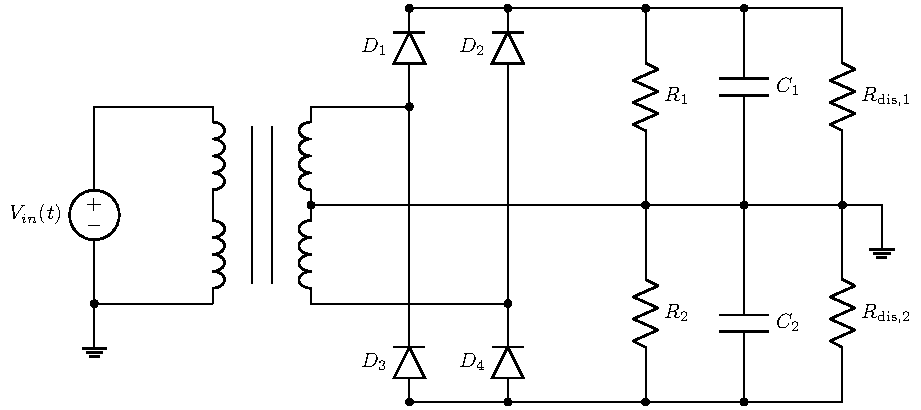
\includegraphics[width=0.75\linewidth]{MainPowerSupply.asc}
    \caption{{Complete schematic of the power supply.}}
    \label{fig:MainPowerSupplySchematic}
\end{figure}
\vspace{10pt}

Figure \ref{fig:MainPowerSupplySchematic} shows the complete schematic of the power supply. Each element in the schematic is clearly labeled and serves a distinct function to meet the defined system requirements.
It is clear from the schematic that the power supply is dependent on multiple factors and parameters and, thus, on their respective value. A brief explanation of these components is provided below. Additional details about their function will be presented in chapter \ref{CircuitDesign}.
\begin{itemize}
    \item {\textbf{Resistors} $R_{1}$ \textbf{and} $R_{2}$}: These resistors will act and form the load of the power supply circuit, therefore simulating the load of real-world scenarios.
    \item {\textbf{Resistors} $R_{\text{dis,1}}$ \textbf{and} $R_{\text{dis},2}$}: These resistors serve as discharge resistors, ensuring the safety of both the users and the capacitors by discharging the stored energy after each power supply operation.
    \item \textbf{Capacitors $C_{1}$ and $C_{2}$}: These capacitors are essential for smoothening the rectified DC output.
    \item \textbf{Diodes (1N5408)}: The diodes in the power supply circuit are responsible for the rectification process, converting the bidirectional flow of alternating current (AC) into the unidirectional flow of direct current (DC). Which is essential for providing a DC voltage output.
\end{itemize}

\subsection{Ripple Voltage}
As mentioned, the smoothing capacitors filter out the ripple from the DC output voltage waveform after the rectifiers. Ripple voltage is a value expressed as a percentage, representing the difference between the maximum and average voltage, divided by the average voltage, and multiplied by 100\%. The formula for calculating the ripple voltage is as follows:

\begin{flalign}\label{Ripple Voltage}
    u_{\text{ripple}}[\%]=\left(\frac{u_{\text{max}}-u_{\text{average}}}{u_{{average}}}\right)\cdot 100\%
\end{flalign}

Further information regarding the ripple voltage and percentage can be found in the subsequent sectors, the Appendix, and the Integrated Project-1 Manual.




\chapter{Design Methodology} 
\label{CircuitDesign}


\section{Design Procedure}
The design procedure for the power supply circuit and system begins with defining the system requirements and a rough understanding of the operating conditions for the Booming Bass Sound System. Most requirements are already addressed in Chapter \ref{CircuitIntroduction}. In brief, the power supply must deliver a stable DC voltage at the positive and negative output terminals, which implies a minimized ripple, particularly under a 1.0 A load current. The target output voltage is $\pm$19 V, with the ripple voltage not exceeding 5\% of its average value.
The primary goal is to design a power supply that efficiently converts the AC voltage from the main outlet through a center-tapped transformer into a stable DC voltage waveform, thus capable of powering and providing power to the entire sound amplifying system.

\subsection{Circuit Component Selection}
With the power supply requirements in mind, the next step was to select appropriate components and to inventory what components were available and required to ensure the operation of the power supply. This included:
\begin{itemize}
    \item \textbf{Transformer}: A center-tapped transformer to provide a dual output voltage necessary for the full wave rectification process. The transformer, therefore, provides both a positive and a negative output.
    \item \textbf{Oscilloscope: Tektronix TDS 2022B} An oscilloscope is necessary to conduct analysis and measurements after building the power supply to check the performance of the power supply.
    \item \textbf{Capacitors}: Smoothing capacitors are used to filter the ripple in the DC output. Since the center-tapped transformer provides both positive and negative outputs at the terminals, two smoothing capacitors are employed- one for the positive voltage and the other for the negative output voltage. 
    \item \textbf{Resistors}: The resistors in the power supply serve different functions; two act as discharge resistors to ensure safe user operation of the power supply, while another two are used to simulate the power supply's load. 
\end{itemize}

\subsection{Analysis, Testing \& Measurements}
The results obtained from simulating the circuit in LTSpice should provide valuable insight into the expected performance of the power supply and what to expect from the power supply.

After analyzing the expected performance of the power supply through circuit simulations, testing and measurements of the assembled power supply must be conducted to verify that its real-world, or in other words practical, performance aligns with the predicted outcomes.

\subsection{Final Design}
If the results align with the requirements of the Booming Bass Project and meet the desired specifications and results, no additional changes and modifications are necessary to the power supply circuit.

\section{Circuit Elements and Components}
The performance of the power supply system depends heavily on design decisions made throughout the project. Achieving the desired performance for the Booming Bass Project requires careful consideration of various factors, such as the selection of diodes, the values of resistors, and the capacitance of smoothing capacitors. Each component's value must be chosen to ensure the power supply meets the specified requirements for voltage regulation, ripple percentage, and load performance. The complete schematic of the circuit is provided in Chapter \ref{CircuitIntroduction}, but for convenience, it is also included here:

\vspace{10pt}
\begin{figure}[h!]
    \centering
    \captionsetup{justification=centering, labelfont=bf}
    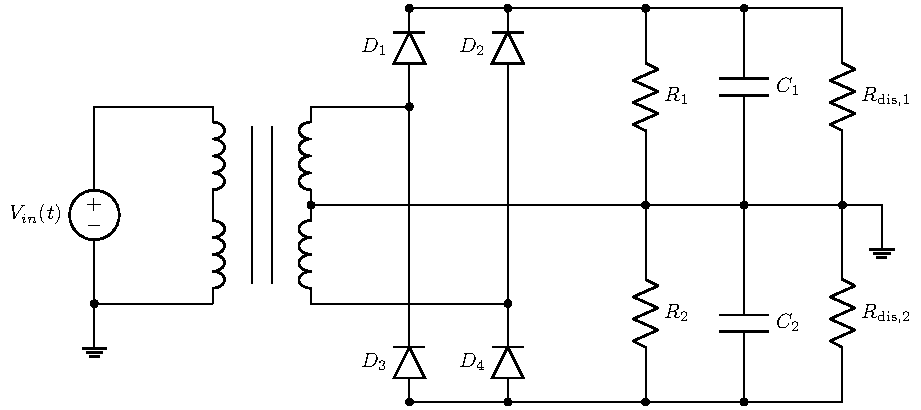
\includegraphics[width=0.75\linewidth]{MainPowerSupply.asc}
    \caption{{Complete schematic of the power supply.}}
    \label{fig:MainPowerSupplySchematic2}
\end{figure}
\vspace{10pt}

The complete schematic of the power supply is shown in Figure \ref{fig:MainPowerSupplySchematic2}. Each element in the schematic is clearly labeled and serves a distinct function to meet the defined system requirements.
It is clear from the schematic that the power supply is dependent on multiple components and, thus, on their respective value.
\begin{itemize}
    \item \textbf{Resistors $R_{1}$ and $R_{2}$}: These resistors act and form the load of the power supply circuit, therefore simulating a real-world load. The values of the load resistors are based on the equivalent resistance of the sound-amplifying system and thus selected to ensure and to check that the output voltage remains within the desired range (e.g., 17-20 V DC) when a load current of 1.0 A is applied to the power supply circuit.
    
    \item {\textbf{Resistors} $R_{\text{dis,1}}$ \textbf{and} $R_{\text{dis,2}}$}: These resistors serve as discharge resistors, ensuring safe operation by discharging the stored energy after power supply operation. These resistors should allow the power supply to be fully discharged within 2.5 minutes after operation
    
    \item \textbf{Capacitors $C_{1}$ and $C_{2}$}: These capacitors are essential for smoothing the rectified AC input, functioning as output filters to reduce ripple in the outgoing DC voltage at each terminal. In the power supply circuit, the AC voltage from the transformer undergoes rectification through the diodes, but fluctuations are still present in the DC output. These fluctuations are referred to as ripple. Capacitors $C_{1}$ and $C_{2}$ charge during the peaks of the DC waveform and discharge during the troughs, effectively ensuring that the DC voltage remains as stable as possible. The difference between the maximum and minimum capacitor voltage is thus called the ripple voltage. The choice of the capacitance values $C_{1}$ and $C_{2}$ and the load current determines the degree of ripple reduction and, thus, the overall stability of the output.
    
    \item \textbf{Diodes (1N5408)}: The power supply circuit diodes are responsible for rectifying the AC input into a unidirectional DC output. The actual diodes are already soldered on and differ from those chosen in the simulation process; the standard 1N4148 diodes are chosen in the LTSpice simulations for convenience.
    While they differ in primary characteristics, the 1N5408 diodes are more resilient than the 1N4148 regarding maximum repetitive peak voltage and maximum RMS voltage.
    
\end{itemize}

\newpage
\subsection{Dimensioning Circuit Components and Elements}
Using the equation provided earlier in Chapter \ref{CircuitIntroduction} and in the Integrated Project-1 Manual for $u_{\text{ripple}}[\%]$, the ripple voltage below 5\%, the maximum voltage can be calculated, assuming that the average voltage after the rectifier is 19  V, given a load current of 1.0 A, as follows:
\begin{flalign}\label{Ripple Voltage2}
    u_{\text{ripple}}[\%]=\left(\frac{u_{\text{max}}-u_{\text{average}}}{u_{{average}}}\right)\cdot 100\%
\end{flalign}

Rearranging equation \ref{Ripple Voltage2} yields the following expression for $u_{\text{max}}$:
\begin{flalign}\label{Maximun Voltage}
    u_{\text{max}}=u_{\text{average}}\left(100\% + u_{\text{ripple}}[\%]\right),\equnit{\si{\volt}}
\end{flalign}

Equation \ref{Maximum Voltage2} remains dependent on the average voltage and the ripple percentage. Therefore, the maximum voltage can be calculated when the average voltage after rectification is 19 V, with a load current of 1.0 A, as shown below:
\begin{flalign}\label{Maximum Voltage2}
u_{\text{max}}  & =u_{\text{average}}\left(100\% + u_{\text{ripple}}[\%]\right)\notag\\
                & = \left(19 V\right)\left({100\% + 5\%}\right)\notag\\
               & = 19.95 V
\end{flalign}

From the calculation, it is clear that the maximum voltage must not exceed 19.95 V to ensure that the ripple voltage remains within 5\% of the average voltage. With this constraint and limitation in place, the necessary capacitance value to keep the ripple voltage under 5\% can be determined and calculated. This calculation is based on a maximum post-rectification voltage of 19 V and during a load current of 1.0 A, using the voltage-current relationship for a capacitor:
\begin{flalign}\label{CapacitorEquation}
    I=C_{1,2}\left(\frac{dV}{dt}\right) 
    \equnit{\si{\ampere}}
\end{flalign}

For this calculation, a first-order approximation of the exponential decay of the voltage across the capacitor is applied. It is assumed that this decay follows a linear behavior, allowing it to be approximated as shown in equation \ref{LinearApproximation}. By combining equations \ref{CapacitorEquation} and \ref{LinearApproximation}, the voltage-current relationship for the capacitor can be rewritten as follows:
\begin{flalign}\label{LinearApproximation}
    \frac{dV}{dt}\approx\frac{\Delta{U_{\text{dc}}}}{\Delta{t}}=\frac{2\left(u_{\text{max}}-u_{\text{average}}\right)}{\Delta t}
\end{flalign}
\begin{flalign}
    I    &= {C_{1,2}}\left(\frac{dV}{dt}\right)={C_{1,2}}\left(\frac{\Delta{U_{\text{dc}}}}{\Delta{t}}\right)=C_{1,2}\left(\frac{2\left(u_{\text{max}}-u_{\text{average}}\right)}{\Delta t}\right) 
    \equnit{\si{\ampere}}
\end{flalign}
The equation for calculating the required capacitance is expressed as:
\begin{flalign}
    C_{1,2}   &=I\left(\frac{1}{\left(\frac{\Delta U_{\text{dc}}}{\Delta t}\right)}\right)=I\left(\frac{\Delta t}{\Delta U_{\text{dc}}}\right)=I\left(\frac{\Delta t}{2\left(u_{\text{max}}-u_{\text{average}}\right)}\right)
    \equnit{\si{F}}
\end{flalign}

Therefore, the required capacitance to achieve a ripple voltage below 5\% is calculated as follows:
\begin{flalign}\label{CapacitorSize} 
C_{1,2}        &= 1.0\left(\frac{0.01}{2(19.95-19.00)}\right)=\left(\frac{0.01}{1.90}\right)= 5.2631\ldots\cdot10^{-3}{F}\notag\\
        &= 5263 \mu{F}
\end{flalign}

It is important to note that the calculated capacitance values apply individually to both the power supply circuit's positive and negative output terminals. Consequently, the two capacitors of equal capacitance are required to ensure proper functionality on either side of the output terminal.

\newpage
\subsubsection{Discharge Resistors}\label{Discharge_Resistor_Section}
For the effective operation of the power supply and to ensure the safety of the smoothing capacitors, discharge resistors play a crucial role. Their value can be determined using the time constant of the power supply, which behaves as an RC circuit. The calculation is based on the following equation, where ${i=1,2}$ respective to each discharge resistor and each smoothing capacitor:

\begin{flalign}\label{RCCircuit}
    \tau    &= {R_{\text{i}}}{C_{\text{i}}}=R_{1,2}C_{1,2}=R_{\text{dis,1 dis,2}}C_{1,2}
    \equnit{\si{s}}
\end{flalign}

As for the power supply circuit, the smoothing capacitors are assumed to be fully discharged after approximately 5$\tau$. Thus, it is assumed that 5$\tau\approx s_{\text{dis}}$, where $s_{\text{dis}}$ represents the discharge time. In this case, the power supply should discharge within 2.5 minutes, meaning that $s_{\text{dis,max}}=150$. Rewriting equation \ref{RCCircuit} for $R_{\text{i}}$ gives:
\begin{flalign}\label{DischargeResistor}
    R_{\text{i}}    &=R_{\text{dis,1 dis,2}}=\frac{\tau}{C_{\text{i}}}=\left(\frac{{\left(\frac{s_{\text{dis}}}{5}\right)}}{C_{\text{i}}}\right)=\frac{s_{\text{dis}}}{5C_{\text{i}}}
    \equnit{\si{\Omega}}
\end{flalign}
Therefore, the discharge resistance required to ensure the power supply fully discharges within 2.5 minutes or 150 seconds is determined as follows:
\begin{flalign}\label{DischargeResistors}
    R_{\text{dis,1. dis,2}}    &=\frac{150}{5(5.263\cdot10^{-3})}\notag\\
                    &=5700 \Omega
\end{flalign}   

A discharge resistance of 5700 $\Omega$ for $R_{\text{dis,1}}$ and $R_{\text{dis,2}}$ respective ensures that the power supply fully discharges within 2.5 minutes, given a smoothing capacitance of 5263 $\mu{F}$ at each side of the output terminals. This calculation and the corresponding equation \ref{DischargeResistor} show that reducing the discharge resistance will result in a shorter discharge time for the power supply. For this reason, a smaller value for the discharge resistor was selected to achieve a shorter discharge time between power supply operations.
\chapter{Simulation results}
\section{LTSpice Simulation}
In this chapter, LTSpice simulations were initialized using the values partially gained from calculations \ref{DischargeResistor} and \ref{CapacitorSize}, although real-world availability of these values wasn't possible. Therefore, deviations were made from the values presented previously; for the capacitor, a value of 6800 $\mu{F}$ was chosen, and for the discharge resistors, a value of 3.9 k$\Omega$ was chosen. Further elaboration and information regarding the choice of values will be presented in the subsequent sections and chapters.
\vspace{10pt}
\begin{figure}[H]
    \centering
    \captionsetup{justification=centering, labelfont=bf}
    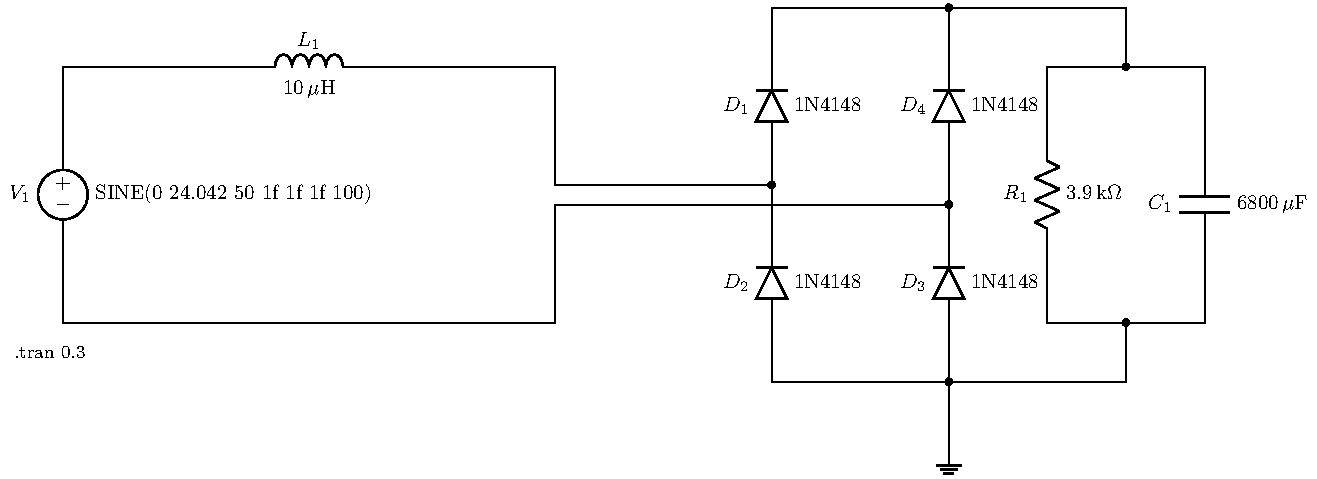
\includegraphics[width=0.8\linewidth]{ps (1).asc}
    \caption{{The LTSpice circuit. For convenience, the transformer is transformed into a  }}
    \label{fig:MainPowerSupplySchematicLTSpice}
\end{figure}

As previously discussed, the LTSpice simulations were performed for only one output terminal, as the use of a center-tapped transformed allows the existence of symmetry of the power supply; this ensures consistent behavior on both the positive and negative output terminals. This means that analysis on only one side of the output terminal is sufficient.

\begin{figure}[H]
    \centering
    \captionsetup{justification=centering, labelfont=bf}
    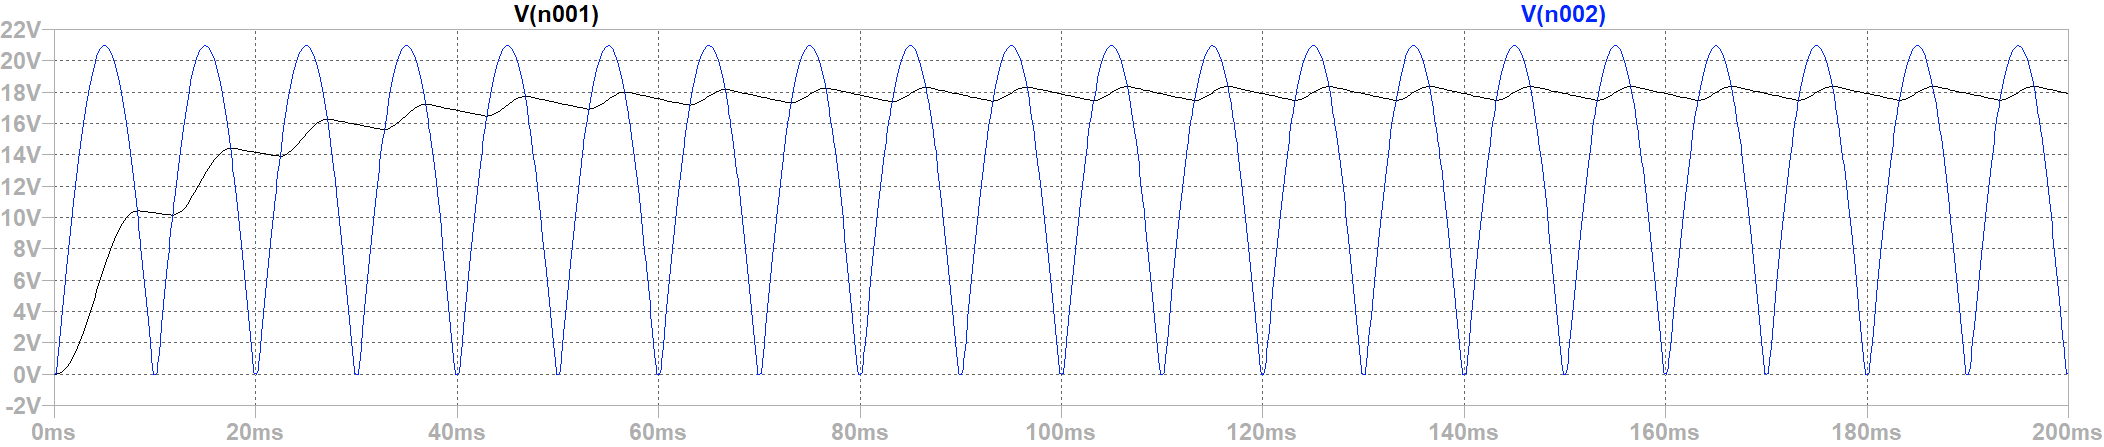
\includegraphics[width=0.98\linewidth]{SimulatedCircuitOutputVoltage}
    \caption{{The simulated circuit output voltage. The blue line represents the circuit without any smoothing capacitors, while the black line represents the circuit with them present.}}
    \label{fig:OutputVoltageWith-Without}
\end{figure}
\begin{figure}[H]
    \centering
    \captionsetup{justification=centering, labelfont=bf}
    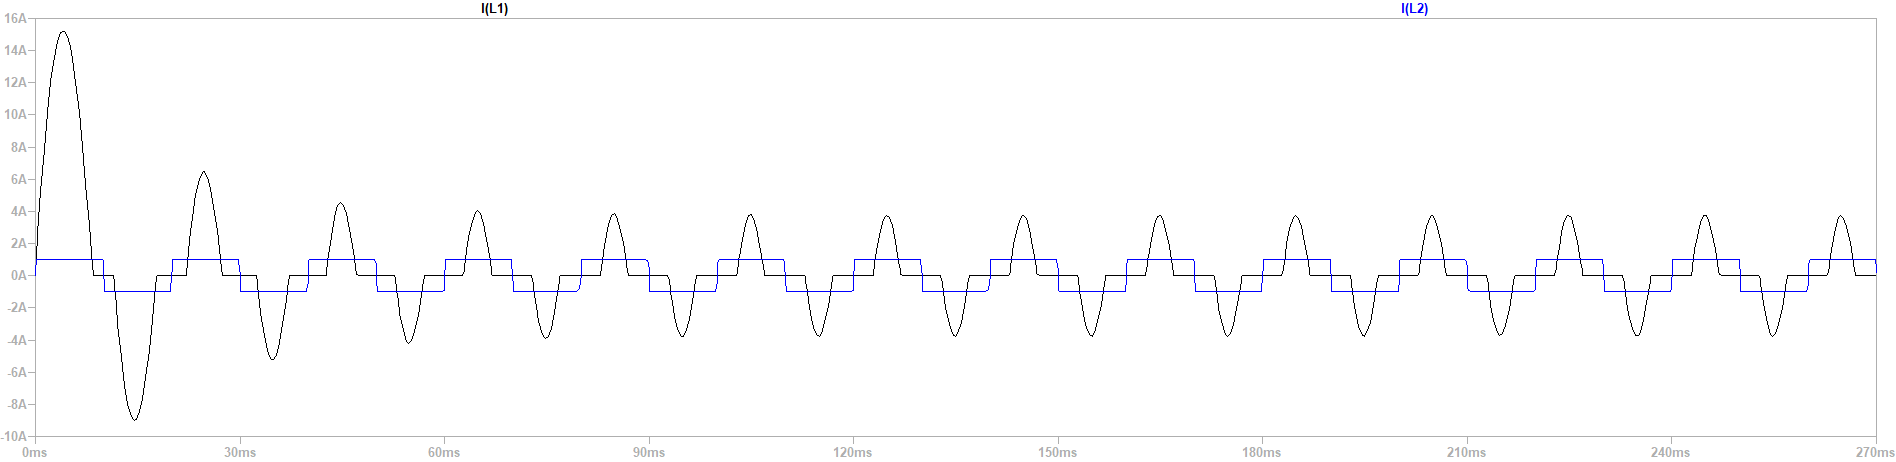
\includegraphics[width=0.98\linewidth]{3}
    \caption{{The simulated circuit current through the transformer. The blue line represents the circuit without any smoothing capacitors, while the black line represents the circuit with them present.}}
    \label{fig:OutputCurrenteWith-Without}
\end{figure}
\vspace{10pt}

Figures \ref{fig:OutputVoltageWith-Without} and \ref{fig:OutputCurrenteWith-Without} clearly demonstrate the impact of the smoothing capacitors on the output voltage and current waveforms. In figure \ref{fig:OutputVoltageWith-Without}, the absence of smoothing capacitors results in the output voltage remaining a somewhat sinusoidal shape even after rectification. Conversely, the inclusion of smoothing capacitors produces an output voltage waveform that closely resembles a steady DC voltage signal. 

\begin{table}[H]
\centering
\captionsetup{justification=centering, labelfont=bf}
\caption{Characteristics of the power supply in simulation under various levels of load.}
\begin{tabularx}{0.8\textwidth}{>{\arraybackslash}X >{\arraybackslash}X >{\arraybackslash}X >{\arraybackslash}X}
    \toprule
    \textbf{Resistance Load [$\Omega$]} & \textbf{Average Voltage [V]} & \textbf{Average Current [A]} & \textbf{Ripple [\%]} \\
    \midrule
    \rowcolor[gray]{.9} {19 $\Omega$} & 18.3 & 0.963 & 0.38 \\
    {38 $\Omega$} & 19.6 & 0.516 & 0.21 \\
    \rowcolor[gray]{.9} {76 $\Omega$} & 20.5 & 0.27 & 0.11 \\
    {Open} & 22.3 & 0.00 & 0.20 \\
    \bottomrule
\end{tabularx}
\label{tab:characteristicsSim}
\end{table}

Table \ref{tab:characteristicsSim} presents the simulation results for the power supply operating under different resistive load conditions. The data includes each load's average output voltage, current, and ripple percentage. The ripple percentage was calculated using equation \ref{Ripple Voltage2}. All the values were calculated by the code in appendix \ref{sec:ripvoltcodesim}. These simulation results demonstrate how the power supply responds to varying loads, providing insight into its ability to maintain consistent performance and stability across different operational scenarios and various load levels.



\chapter{Power Supply Assembly}
\section{Main Power Supply PCB}
This chapter outlines the step-by-step process for assembling the power supply circuit, ensuring accurate implementation of all components and elements. The Power Supply Assembly procedure includes soldering on the smoothing capacitors $C_{1}$ and $C_{2}$ and the discharge resistors $R_{\text{dis,1}}$ and $R_{\text{dis,2}}$. The selection and dimensioning of each component within the power supply circuit have been thoroughly addressed in the preceding sections of this report.

\vspace{10pt}
\begin{figure}[h!]
    \centering
    \captionsetup{justification=centering, labelfont=bf}
    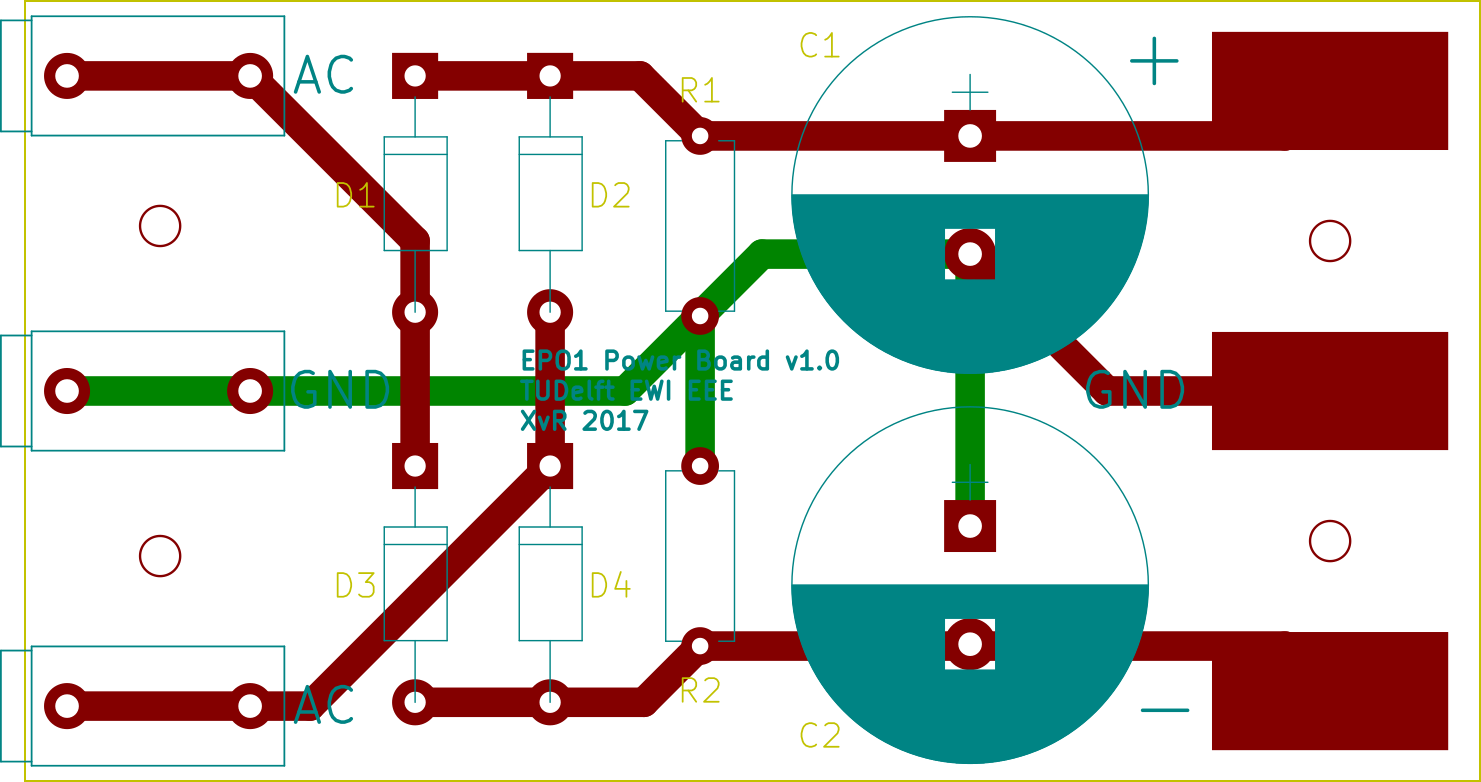
\includegraphics[width=0.75\linewidth]{21}
    \caption{{The layout of the power supply PCB. The positions in yellow and cyan correspond to the respective names of the components used in this report.}}
    \label{fig:MainPowerSupplySchematicPCB}
\end{figure}
\vspace{10pt}
The PCB layout below clearly illustrates the designated locations for each component discussed, where the diodes responsible for the rectification process were pre-soldered. The power supply's positive and negative output terminals are located on the right side of the circuit, as seen in figure \ref{fig:MainPowerSupplySchematicPCB}, relative to the ground on the same side.

\subsection{The Smoothing Capacitors}
As previously discussed in Chapter \ref{CircuitIntroduction} and Chapter \ref{CircuitDesign}, the capacitors in the power supply are used to smoothen out the voltage waveform after rectification. The capacitors achieve this by storing energy during the peaks of the DC voltage waveform and releasing it during the troughs, effectively reducing the fluctuations and, therefore, ensuring a more stable output voltage. Based on calculations \ref{Maximum Voltage2} and \ref{CapacitorSize} in chapter \ref{CircuitDesign}, it is evident that a capacitance of 5263 $\mu{F}$ is required on each output terminal of the power supply to maintain ripple voltage below 5\%. 

In reality, the available capacitor values options were limited to one for 4700 $\mu{F}$ and another option for 6800 $\mu{F}$. Still, as previously discussed, a higher capacitance results in reduced ripple, leading to a more stable DC output voltage waveform. The capacitance's value is important since it directly dictates the magnitude of the smoothening. A higher capacitance ensures a more stable output voltage waveform. For this reason, the 6800 $\mu{F}$ capacitor was chosen as the smoothing capacitors.

\subsection{Discharge Resistors}
As previously discussed in Chapter \ref{CircuitDesign} and section \ref{Discharge_Resistor_Section}, the discharge resistors in the power supply are responsible for the safe discharge of the power supply operation. Based on calculation \ref{DischargeResistors}, it is evident that a resistance of 5700 $\Omega$ is required. However, as discussed in section \ref{Discharge_Resistor_Section}, a smaller value of the discharge resistor contributes to a shorter overall discharge time and, therefore, quicker times between operation sessions. For this exact reason, a 3.9 k$\Omega$ resistor is used.

\subsection{The Load Resistors}
Load resistors were utilized to simulate a load current of 1.0 A on the power supply circuit while maintaining a rectified voltage of 19 V. These components were readily available and required minimal handling by connection via banana cables for integration to the power supply.


\chapter{Measurement results } 

Multiple measurements were done to characterize the power supply and to measure its performance. The following characteristics and scenarios were measured:
\begin{itemize}
    \item The average output voltage under various levels of load.
    \item The ripple in the output voltage under various levels of load.
    \item The capacitors' discharge time after power supply operation. 
\end{itemize} 

\section{Average Voltage and Ripple}

The voltage waveform across the load resistors $R_{1}$ and $R_{2}$ was measured under four distinct conditions to evaluate the ripple voltage. These measurements aimed to analyze the behavior of the power supply under varying load scenarios, where $R_{\text{1}}$ and $R_{\text{2}}$ simulate the operational load conditions of the circuit. The table below outlines the different test conditions:

\begin{table}[h!]
\centering
\captionsetup{justification=centering, labelfont=bf}
\caption{\textbf{Different conditions Ripple Voltage.}}
\begin{tabular*}{0.9\textwidth}{@{\extracolsep{\fill}} p{0.8\textwidth} @{}} 
\toprule
    \begin{itemize}
        \item \textbf{Resistors in Series} \newline With the output terminals connected to two 38 $\Omega$ resistors in series, thus forming a 19 $\Omega$ resistor as an equivalent resistor.
        \item \textbf{Single Resistor} \newline With the output terminals connected to a single 38 $\Omega$ resistor.
        \item \textbf{Resistor in Parallel} \newline With the output terminals connected to two 38 $\Omega$ resistors in parallel, forming a 76 $\Omega$ resistor as an equivalent resistor.
        \item \textbf{No Load Resistors} \newline With no load on the output terminals.
    \end{itemize} \\
     \bottomrule
\end{tabular*}
\label{ConditionsRippleVoltage}
\end{table}

The graphs of the measurements can be seen in appendix \ref{sec:ripple}. When conducting those measurements, only the positive side of the power supply was loaded because the negative side is an exact copy of the positive one. Support for this claim in practice can be found in appendix \ref{sec:practevidencesymmetry}. Those measurements were done by connecting the probe to the ground and the positive output of the power supply (and by measuring the voltage over the resistors).

Those measurements led to the characteristics seen in table \ref{tab:characteristics}. The ripple was calculated using the following formula \cite{labmanual}:
\begin{flalign*}
    u_{\text{ripple}}[\%]=\left(\frac{u_{\text{max}}-u_{\text{average}}}{u_{{average}}}\right)\cdot 100\%\
\end{flalign*}
The code in appendix \ref{sec:ripvoltcodemea} was used to calculate the values in table \ref{tab:characteristics}. 

The ripple for the open circuit is most likely just a measurement error of the oscilloscope because the oscilloscope was set to have a resolution of 0.04 V. In the measurements, the maximum voltage is 23.04 V, and the average voltage is 23.00 V. Although there would have been a small ripple due to the capacitors slowly discharging through the discharge resistor, the ripple induced by this current was insignificant compared to the one measured, as the discharge current is very small.

\begin{table}[H]
\centering
\captionsetup{justification=centering, labelfont=bf}
\caption{Characteristics of the power supply under various levels of load.}
\begin{tabularx}{0.8\textwidth}{>{\arraybackslash}X >{\arraybackslash}X >{\arraybackslash}X >{\arraybackslash}X}
    \toprule
    \textbf{Resistance Load [$\Omega$]} & \textbf{Average Voltage [V]} & \textbf{Average Current [A]} & \textbf{Ripple [\%]} \\
    \midrule
    \rowcolor[gray]{.9} {19 $\Omega$} & 20.1 & 1.06 & 3.23 \\
    {38 $\Omega$} & 21.1 & 0.56 & 1.66 \\
    \rowcolor[gray]{.9} {76 $\Omega$} & 21.9 & 0.29 & 1.19 \\
    {Open} & 23.0 & 0.00 & 0.29 \\
    \bottomrule
\end{tabularx}
\label{tab:characteristics}
\end{table}


As can be seen by comparing the simulation table with the table above, it is clear that there is a significant discrepancy between the simulation and measurement results. This can be attributed to various factors:
\begin{itemize}
    \item The diodes used in the simulation differ from those used in reality. The 1N4148 diodes used in the simulation are general diodes and are not fitted to carry large currents \cite{1n4148}. The 1N5408, on the contrary, can carry average rectified currents up to 3.0 A \cite{1n5408}.
\end{itemize}

\section{Discharge Time Capacitors}

\begin{figure}[H]
    \centering
    \captionsetup{justification=centering, labelfont=bf}
    \resizebox{0.8\columnwidth}{!}{%
        \begin{tikzpicture} 
                \begin{axis} [xlabel=Time (s), ylabel=Voltage (V)]
                    \addplot+[no markers] table [x=d, y=e, col sep=comma] {./csv/discharge/F0010CH1.CSV};
                    \addlegendentry{\(V_{out}\)}
                    \addplot[color=red] table[row sep = crcr]{0 8.829 \\ 249.8 8.829 \\};
                    \addplot[green, dotted] table[row sep = crcr]{33 0 \\ 33 25 \\};
                    \addplot[green, dotted] table[row sep = crcr]{62 0 \\ 62 25 \\};
                    \addlegendentry{\(V_{e^-1}\)}
                \end{axis}
        \end{tikzpicture}%
    }
    \caption{The discharge curve of the capacitors.}
    \label{fig:dischargeCurve}
\end{figure}

From figure \ref{fig:dischargeCurve}, it can be seen that the capacitors are disconnected from the power supply at \(t=33.0s\). The curve crosses the red line (which indicates the point that \(\tau\) is 1) at \(t\approx 62s\). This means \(\tau \approx 28s\), which means that the capacitors will be discharged after 145 seconds, which fits nicely in the 2.5-minute limit it was designed for.


\printbibliography

%% Use letters for the chapter numbers of the appendices.

%\input{appendix-a}
 
\appendix
\chapter{Appendix }
This chapter presents additional tips and resources.  
\section{Tips}
The students should prepare the reports in a proper format. This means that they should use commonly accepted font and font size, page margins, heading sizes etc. Graphs and tables should be legible on paper (after printing), should have captions in a matching style, etc. They should not forget to include cover, title page, table of contents for the report.\par 
A suggested template is provided on overleaf  \href{https://www.overleaf.com/read/xdynzwbcdvzy
}{\color{tudelft-cyan}{https://www.overleaf.com/read/xdynzwbcdvzy
}}

\section{Resources}
You may also use the  \LaTeX templates provided in the sources listed below:
\begin{itemize}
    \item TU Delft corporate identity page page provides additional resources for \LaTeX: \\ \href{https://www.tudelft.nl/huisstijl/downloads}{\color{tudelft-cyan}{www.tudelft.nl/huisstijl/downloads}}
    \item Overleaf also presents additional template options: \href{https://www.overleaf.com/edu/tudelft#templates}{\color{tudelft-cyan}{www.overleaf.com/edu/tudelft\#templates}}
\end{itemize}
\chapter{Simulations}

\section{Average Voltage and Ripple Simulation Results}
\label{sec:ripplesimulation}

Can be seen in local

\chapter{Measurements}

\section{Average Voltage and Ripple Measurement Results}
\label{sec:ripple}

\begin{figure}[H]
    \centering
    \captionsetup{justification=centering, labelfont=bf}
    \resizebox{0.8\columnwidth}{!}{%
        \begin{tikzpicture} 
                \begin{axis} [xlabel=Time (s), ylabel=Voltage (V)]
                    \addplot table [x=d, y=e, col sep=comma, mark=none] {./csv/19 ohm/F0009CH1.CSV};
                \end{axis}
        \end{tikzpicture}%
    }
    \caption{The output voltage waveform with the power supply loaded with a 19 \(\Omega\) resistor.}
    \label{fig:ripple19ohm}
\end{figure}
\begin{figure}[H]
    \centering
    \captionsetup{justification=centering, labelfont=bf}
    \resizebox{0.8\columnwidth}{!}{%
        \begin{tikzpicture} 
                \begin{axis} [xlabel=Time (s), ylabel=Voltage (V)]
                    \addplot table [x=d, y=e, col sep=comma, mark=none] {./csv/38 ohm/F0007CH1.CSV};
                \end{axis}
        \end{tikzpicture}%
    }
    \caption{The output voltage waveform with the power supply loaded with a 38 \(\Omega\) resistor.}
    \label{fig:ripple38ohm}
\end{figure}
\begin{figure}[H]
    \centering
    \captionsetup{justification=centering, labelfont=bf}
    \resizebox{0.8\columnwidth}{!}{%
        \begin{tikzpicture} 
                \begin{axis} [xlabel=Time (s), ylabel=Voltage (V)]
                    \addplot table [x=d, y=e, col sep=comma, mark=none] {./csv/76 ohm/F0011CH1.CSV};
                \end{axis}
        \end{tikzpicture}%
    }
    \caption{The output voltage waveform with the power supply loaded with a 76 \(\Omega\) resistor.}
    \label{fig:ripple76ohm}
\end{figure}
\begin{figure}[H]
    \centering
    \captionsetup{justification=centering, labelfont=bf}
    \resizebox{0.8\columnwidth}{!}{%
        \begin{tikzpicture} 
                \begin{axis}[voltageToZero]
                    \addplot table [x=d, y=e, col sep=comma, mark=none] {./csv/No load/F0008CH1.CSV};
                \end{axis}
        \end{tikzpicture}%
    }
    \caption{The output voltage waveform with no load on the output terminals.}
    \label{fig:outputopen}
\end{figure}

\newpage

\section{Symmetry of Power Supply}
\label{sec:practevidencesymmetry}

To show that the claim that the negative part of the power supply is the mirrored counterpart of the positive part also holds in practice, some measurements were conducted. In figure \ref{fig:ripple38ohmboth}, a 38 \\Omega resistor was connected between the positive output and ground and the negative output and ground. This figure shows that the positive output mirrored around 0 V equals the negative output. Figure \ref{fig:outputopenboth} shows this too.

\begin{figure}[H]
    \centering
    \captionsetup{justification=centering, labelfont=bf}
    \resizebox{0.8\columnwidth}{!}{%
        \begin{tikzpicture} 
                \begin{axis} [xlabel=Time (s), ylabel=Voltage (V)]
                    \addplot table [x=d, y=e, col sep=comma, mark=none] {./csv/38 ohm/F0007CH1.CSV};
                    \addplot table [x=d, y=e, col sep=comma, mark=none] {./csv/38 ohm/F0007CH2.CSV};
                \end{axis}
        \end{tikzpicture}%
    }
    \caption{The output voltage waveform with the power supply loaded with a 38 \(\Omega\) resistor.}
    \label{fig:ripple38ohmboth}
\end{figure}

\begin{figure}[H]
    \centering
    \captionsetup{justification=centering, labelfont=bf}
    \resizebox{0.8\columnwidth}{!}{%
        \begin{tikzpicture} 
                \begin{axis} [xlabel=Time (s), ylabel=Voltage (V)]
                    \addplot table [x=d, y=e, col sep=comma, mark=none] {./csv/No load/F0008CH1.CSV};
                    \addplot table [x=d, y=e, col sep=comma, mark=none] {./csv/No load/F0008CH2.CSV};
                \end{axis}
        \end{tikzpicture}%
    }
    \caption{The output voltage waveform with the power supply under no load.}
    \label{fig:outputopenboth}
\end{figure}


\chapter{Code}
\label{ch:code}

\section{Ripple and Average Voltage Simulations}
\label{sec:ripvoltcodesim}

Below code was used to calculate the average voltage and ripple of the output voltage of the simulations.

\begin{python}
import pandas as pd

def ripple(avg, max):
    return (max-avg)/avg*100


datas = [(".\\19 ohm.txt",19),
    	(".\\38 ohm.txt",38),
    	(".\\76 ohm.txt",76),
    	(".\\no load.txt",None)]

for data in datas:
    file = data[0]
    resistance = data[1]
    
    data = pd.read_csv(file, delimiter="\t")
    #Only take the last part of the simulation to avoid the waveform when the capacitors are still being loaded
    t = data["time"][len(data["time"])//3*2:]
    v = data["V(n001)"][len(data["V(n001)"])//3*2:]
    i = data["I(R2)"][len(data["I(R2)"])//3*2:]

    maxV = v.max()
    minV = v.min()
    meanV = v.mean()
    meanI = i.mean()
    
    if resistance == None:
        print(f"Using {file} (Power supply is not loaded)")
    else:
        print(f"Using {file} (Power supply is loaded with a {resistance} Ohm resistor)")

    print(f"    Load resistance: {resistance}")   
    print(f"    Average Voltage: {meanV:.3}V")
    print(f"    Average Current: {meanI:.3}A")
    print(f"    Ripple: {ripple(meanV, maxV):.3}%")
\end{python}
\newpage
\section{Ripple and Average Voltage Measurements}
\label{sec:ripvoltcodemea}

Below code was used to calculate the average voltage and ripple of the output voltage of the measurements.

\begin{python}
import pandas as pd

def ripple(avg, max):
    return (max-avg)/avg*100

# Tuples are formatted as (filename,resistance)
datas = [(".\\19 ohm\\F0009CH1.CSV",19),
    	(".\\38 ohm\\F0007CH1.CSV",38),
    	(".\\76 ohm\\F0011CH1.CSV",76),
    	(".\\No load\\F0008CH1.CSV",None)]

for data in datas:
    file = data[0]
    resistance = data[1]
    
    measured_data = pd.read_csv(file, usecols=[3,4])
    t = measured_data["d"]
    v = measured_data["e"]

    maxV = v.max()
    minV = v.min()
    meanV = v.mean()

    if resistance == None:
        print(f"Using {file} (Power supply is not loaded)")
    else:
        print(f"Using {file} (Power supply is loaded with a {resistance} Ohm resistor)")
    print(f"    Load resistance: {resistance}")   
    print(f"    Average Voltage: {meanV:.3}V")
    if resistance == None:
        print(f"    Average Current: 0.00A")
    else:
        print(f"    Average Current: {meanV/resistance:.3}A")
    print(f"    Ripple: {ripple(meanV, maxV):.3}%")

\end{python}



\end{document}

